\documentclass[12pt,letterpaper]{article}
\usepackage{graphicx,textcomp}
\usepackage{natbib}
\usepackage{setspace}
\usepackage{fullpage}
\usepackage{color}
\usepackage[reqno]{amsmath}
\usepackage{amsthm}
\usepackage{fancyvrb}
\usepackage{amssymb,enumerate}
\usepackage[all]{xy}
\usepackage{endnotes}
\usepackage{lscape}
\newtheorem{com}{Comment}
\usepackage{float}
\usepackage{hyperref}
\newtheorem{lem} {Lemma}
\newtheorem{prop}{Proposition}
\newtheorem{thm}{Theorem}
\newtheorem{defn}{Definition}
\newtheorem{cor}{Corollary}
\newtheorem{obs}{Observation}
\usepackage[compact]{titlesec}
\usepackage{dcolumn}
\usepackage{tikz}
\usetikzlibrary{arrows}
\usepackage{multirow}
\usepackage{xcolor}
\newcolumntype{.}{D{.}{.}{-1}}
\newcolumntype{d}[1]{D{.}{.}{#1}}
\definecolor{light-gray}{gray}{0.65}
\usepackage{url}
\usepackage{listings}
\usepackage{color}

\definecolor{codegreen}{rgb}{0,0.6,0}
\definecolor{codegray}{rgb}{0.5,0.5,0.5}
\definecolor{codepurple}{rgb}{0.58,0,0.82}
\definecolor{backcolour}{rgb}{0.95,0.95,0.92}

\lstdefinestyle{mystyle}{
	backgroundcolor=\color{backcolour},   
	commentstyle=\color{codegreen},
	keywordstyle=\color{magenta},
	numberstyle=\tiny\color{codegray},
	stringstyle=\color{codepurple},
	basicstyle=\footnotesize,
	breakatwhitespace=false,         
	breaklines=true,                 
	captionpos=b,                    
	keepspaces=true,                 
	numbers=left,                    
	numbersep=5pt,                  
	showspaces=false,                
	showstringspaces=false,
	showtabs=false,                  
	tabsize=2
}
\lstset{style=mystyle}
\newcommand{\Sref}[1]{Section~\ref{#1}}
\newtheorem{hyp}{Hypothesis}

\title{Problem Set 2}
\date{Due: February 18, 2024}
\author{Applied Stats II}


\begin{document}
	\maketitle
	\section*{Instructions}
	\begin{itemize}
		\item Please show your work! You may lose points by simply writing in the answer. If the problem requires you to execute commands in \texttt{R}, please include the code you used to get your answers. Please also include the \texttt{.R} file that contains your code. If you are not sure if work needs to be shown for a particular problem, please ask.
		\item Your homework should be submitted electronically on GitHub in \texttt{.pdf} form.
		\item This problem set is due before 23:59 on Sunday February 18, 2024. No late assignments will be accepted.
	%	\item Total available points for this homework is 80.
	\end{itemize}

	
	%	\vspace{.25cm}
	
%\noindent In this problem set, you will run several regressions and create an add variable plot (see the lecture slides) in \texttt{R} using the \texttt{incumbents\_subset.csv} dataset. Include all of your code.

	\vspace{.25cm}
%\section*{Question 1} %(20 points)}
%\vspace{.25cm}
\noindent We're interested in what types of international environmental agreements or policies people support (\href{https://www.pnas.org/content/110/34/13763}{Bechtel and Scheve 2013)}. So, we asked 8,500 individuals whether they support a given policy, and for each participant, we vary the (1) number of countries that participate in the international agreement and (2) sanctions for not following the agreement. \\

\noindent Load in the data labeled \texttt{climateSupport.RData} on GitHub, which contains an observational study of 8,500 observations.

\begin{itemize}
	\item
	Response variable: 
	\begin{itemize}
		\item \texttt{choice}: 1 if the individual agreed with the policy; 0 if the individual did not support the policy
	\end{itemize}
	\item
	Explanatory variables: 
	\begin{itemize}
		\item
		\texttt{countries}: Number of participating countries [20 of 192; 80 of 192; 160 of 192]
		\item
		\texttt{sanctions}: Sanctions for missing emission reduction targets [None, 5\%, 15\%, and 20\% of the monthly household costs given 2\% GDP growth]
		
	\end{itemize}
	
\end{itemize}

\newpage
\noindent Please answer the following questions:

\begin{enumerate}
	\item
	Remember, we are interested in predicting the likelihood of an individual supporting a policy based on the number of countries participating and the possible sanctions for non-compliance.
	\begin{enumerate}
		\item [] Fit an additive model. Provide the summary output, the global null hypothesis, and $p$-value. Please describe the results and provide a conclusion.
		%\item
		%How many iterations did it take to find the maximum likelihood estimates?
		
		\vspace{3cm}
		
		\texttt{Answer}:
		
		\vspace{.5cm}
		
		\lstinputlisting[language=R, firstline=43,lastline=62]{PS2.R} 
		
		\begin{figure}[H] 
			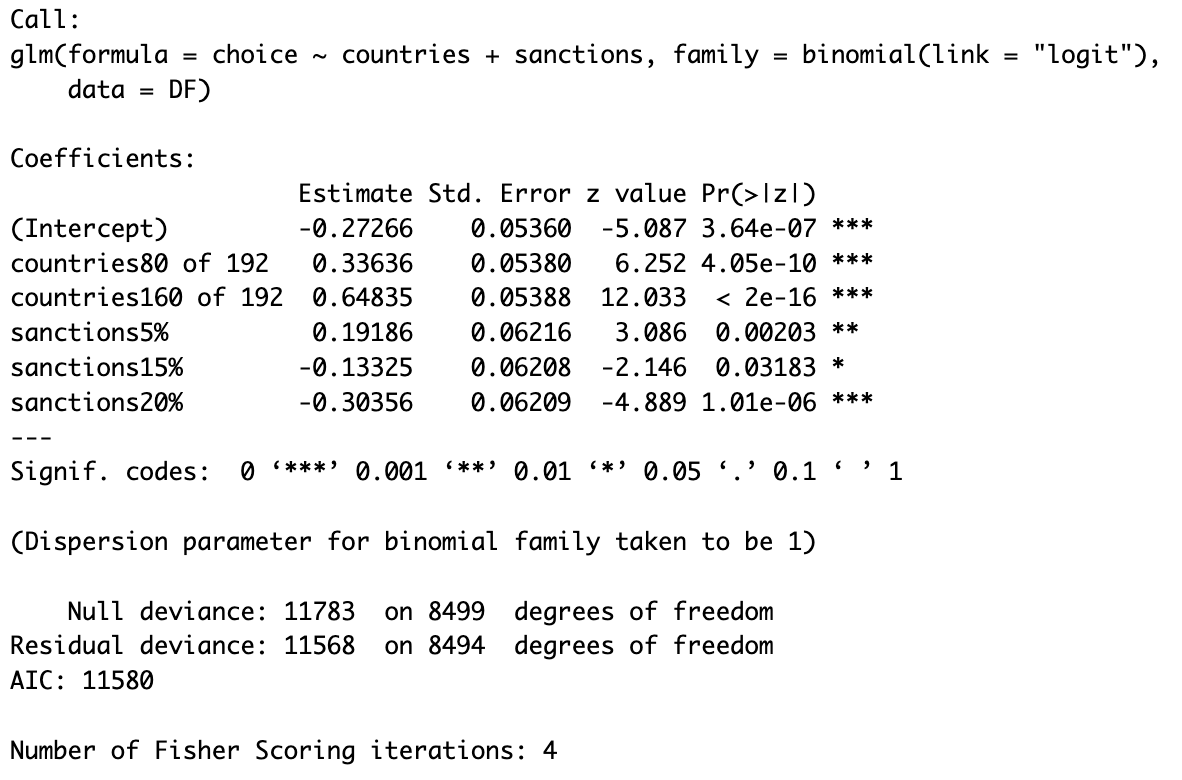
\includegraphics[width=0.7\textwidth]{logit1.png} 
			\caption{logit} 
		\end{figure}
		
		\vspace{.5cm}
	\texttt{The global null hypothesis and p-value}: the global null hypothesis is that efficient equals to 0.the p-value for the coefficient of countries80 of 192 is 4.05e-10, the null hypothesis is that the coefficient = 0, that is, is the average difference on log-odds value between countries80 of 192 and countries20 of 192 is 0. The p-value for the coefficient of countries160 of 192 is < 2e-16, the null hypothesis is that the coefficient = 0, that is, is the average difference on log-odds value between countries160 of 192 and countries20 of 192 is 0. the p-value for the coefficient of sanctions5\%  is 0.00203, the null hypothesis is  that the coefficient = 0, that is, is the average difference on log-odds value between sanctions5\% and None is 0. The p-value for the coefficient of sanctions15\%  is 0.03183, the null hypothesis is  that the coefficient = 0, that is, is the average difference on log-odds value between sanctions15\% and None is 0. The p-value for the coefficient of sanctions20\%  is 1.01e-06, the null hypothesis is  that the coefficient = 0, that is, is the average difference on log-odds value between sanctions20\% and None is 0.Conclusion: All coefficient are significantly not equal to 0. Thus, we get the predicion equation:
		
		\vspace{.5cm}
		
		\texttt{Equation}: log(odds)=-0.27266+0.33636*D(countries80 of 192)+0.64835*D(countries160 of 192)  +0.19186*D(sanctions5\% )-0.13325*D(sanctions15\%)-0.30356*D(sanctions20\%)
				\vspace{3cm}
	\end{enumerate}
	
	\item
	If any of the explanatory variables are significant in this model, then:
	\begin{enumerate}
		\item
		For the policy in which nearly all countries participate [160 of 192], how does increasing sanctions from 5\% to 15\% change the odds that an individual will support the policy? (Interpretation of a coefficient)
%		\item
%		For the policy in which very few countries participate [20 of 192], how does increasing sanctions from 5\% to 15\% change the odds that an individual will support the policy? (Interpretation of a coefficient)

	\vspace{3cm}

\texttt{Answer}:

\vspace{.5cm}

\texttt log(odds)=-0.27266+0.33636*D(countries80 of 192)+0.64835*D(countries160 of 192)     +0.19186*D(sanctions5\% )-0.13325*D(sanctions15\%)-0.30356*D(sanctions20\%) 

\vspace{.5cm}

\texttt When countries participate [160 of 192] and sanctions is 5\%, the equation is log(odds)=-0.27266+0.64835+0.19186=0.56755 
odds=exp(0.56755)=1.76394 

\vspace{.5cm}

\texttt When countries participate [160 of 192] and sanctions is 15\%, the equation is log(odds)=-0.27266+0.64835-0.13325=0.24244
odds=exp(0.24244)=1.274355 

\vspace{.5cm}

\texttt The change in odds is 1.274355-1.76394=-0.489585 

\vspace{.5cm}

\texttt The change in log-odds equals to the coefficient of D(sanctions15\%) minus the coefficient of D(sanctions5\%), so the change in odds is -0.489585

\vspace{3cm}
\
		\item
		What is the estimated probability that an individual will support a policy if there are 80 of 192 countries participating with no sanctions? 
		
			\vspace{4cm}
		
		\texttt{Answer}:
		
		\vspace{.5cm}
		
		if there are 80 of 192 countries participating with no sanctions log(odds)=-0.27266+0.33636=0.0637  p=exp(log(odds))/(1+exp(log(odds)))=0.5159196 the estimated probability that an individual will support a policy if there are 80 of 192 countries participating with no sanctions is 0.5159196
		
			\vspace{3cm}
		
		\item
		Would the answers to 2a and 2b potentially change if we included the interaction term in this model? Why? 
		\begin{itemize}
			\item Perform a test to see if including an interaction is appropriate.
		\end{itemize}
		
		\vspace{3cm}
	
	\texttt{Answer}:
	
	\vspace{.5cm}
		
		\texttt	Yes, the answers to 2a and 2b would potentially change if we included the interaction term in this model, because when an interaction term is included in the model, it allows for the possibility that the effect of one predictor on the outcome variable depends on the level of another predictor. This means that the relationship between one predictor and the outcome variable is not constant across different levels of the other predictor. As a result, the interpretation of the coefficients associated with each predictor becomes more complex, as the effect of one predictor depends on the level of the other predictor.


	
	\texttt  The P-value of chisq-test bigger than 0.05, which means we cannot reject the null hypothesis  that the equation including interaction items cannot perform better significantly than equatio not including those . Therefore, including an interaction is not appropriate.
	
\begin{lstlisting}[language=R]
logit1 <- glm(choice ~ countries+sanctions, family = binomial(link = "logit"), data = DF)
logit2 <- glm(choice ~ countries+sanctions+countries:sanctions, family = binomial(link = "logit"), data = DF)
anova (logit1, logit2,test="Chisq")\end{lstlisting}
\begin{figure}[H] 
	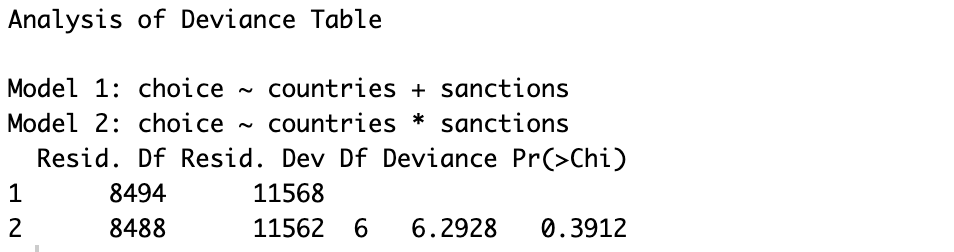
\includegraphics[width=0.7\textwidth]{Anova.png} 
	\caption{Anova} 
\end{figure}
	
	\end{enumerate}
	\end{enumerate}


\end{document}
